\begin{frame}
	\myheading{Module 3.1: Sigmoid Neuron}
\end{frame}

\begin{frame}
	\begin{block}{The story ahead ...}
		\begin{itemize}\justifying
			\item<1-> Enough about boolean functions!
			\item<2-> What about arbitrary functions of the form $y=f(x)$ where $x\in \mathbb{R}^n$ (instead of $\{0, 1\}^n$) and $y \in \mathbb{R}$ (instead of $\{0, 1\}$) ?
			\item<3-> Can we have a network which can (approximately) represent such functions ?
			\item<4-> Before answering the above question we will have to first graduate from \textbf{\textit{perceptrons}} to \textbf{\textit{sigmoidal neurons}} ...
		\end{itemize}
	\end{block}
\end{frame}

\begin{frame}
	\begin{block}{Recall}
		\begin{itemize}\justifying
			\item A perceptron will fire if the weighted sum of its inputs is greater than the threshold (-$w_0$)
		\end{itemize}
	\end{block}
\end{frame}

\begin{frame}
	\begin{columns}
		\column{0.4\textwidth}
		\begin{overlayarea}{\textwidth}{\textheight}
			\begin{center}
				
\begin{tikzpicture}
	\node (input2) at (10,-0.1)  {$x_{1}$};
	\node [hidden_neuron] (neuron1) at (10,2)  {};
	\node (output0)  at (10,3.5) {$y$};
	\draw [->] (input2) -- (neuron1);
	\draw [->] (neuron1) -- (output0);
	\node (bias) at (8, 2) {$bias = w_0 = -0.5$};
	\node (weight) at (9.4,0.6) {$w_1 = 1$};
	\onslide<3->{\node (text) at (10,-0.7) {$criticsRating$};}
\end{tikzpicture}
			\end{center}
		\end{overlayarea}
		\column{0.6\textwidth}
		\begin{overlayarea}{\textwidth}{\textheight}
			\begin{itemize}\justifying
				\item<1-> The thresholding logic used by a perceptron is very harsh !
				\item<2-> For example, let us return to our problem of deciding whether we will like or dislike a movie
				\item<3-> Consider that we base our decision only on one input ($x_1 = criticsRating$ which lies between 0 and 1)
				\item<4-> If the threshold is 0.5 ($w_0 = -0.5$) and $w_1 = 1$ then what would be the decision for a movie with $criticsRating=0.51$ ? \onslide<5->{(like)}
				\item<6-> What about a movie with $criticsRating=0.49$ ? \onslide<7->{(dislike)}
				\item<8-> It seems harsh that we would like a movie with rating 0.51 but not one with a rating of 0.49
			\end{itemize}
		\end{overlayarea}
	\end{columns}
\end{frame}

\begin{frame}
	\begin{columns}
		\column{0.4\textwidth}
		\begin{overlayarea}{\textwidth}{\textheight}
			\begin{center}
				\only<2-4>{
					\input{modules/Module1/tikz_images/only_sign}
				}
				\only<5->{
					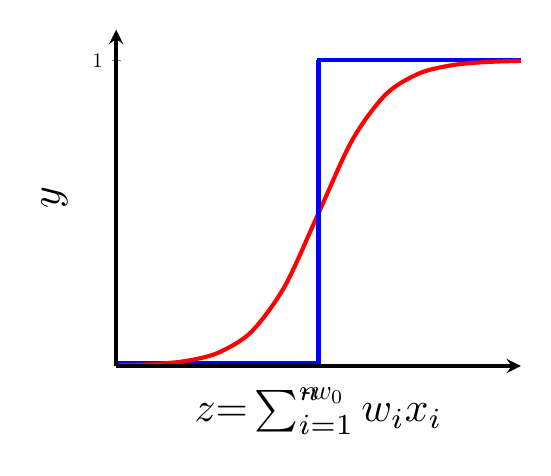
\begin{tikzpicture}[scale=0.75]
	\begin{axis}[
			xmin=-2.5, xmax=2.5,
			ymin=-0.0, ymax=1.1,
			axis lines=left,
			xtick=\empty, ytick={1},
			axis on top=true,
			line width = 2pt,
			%domain=-2.5:2.5,
			ylabel=$y$,
			xlabel=$z{=}\sum_{i=1}^{n} w_i x_i$,
			label style={scale=2}
		]

		\addplot[line width = 5pt, domain=-2.5:0,blue] {0};
		\addplot[line width = 2pt, domain=-0.02:2.5,blue] {1};

		\addplot [smooth,line width = 2pt, mark=none,draw=red] {1/(1+exp(-2.5*\x)};

		\draw[line width=2pt, blue] (axis cs:0,0) -- (axis cs:0,1);
		%% Add the asymptotes
	\end{axis}

	\node at (3.5,-0.5) {-$w_0$};
\end{tikzpicture}
				}
			\end{center}
		\end{overlayarea}
		\column{0.6\textwidth}
		\begin{overlayarea}{\textwidth}{\textheight}
			\only<1-4>{
				\begin{itemize}\justifying
					\item<1-> This behavior is not a characteristic of the specific problem we chose or the specific weight and threshold that we chose
					\item<2-> It is a characteristic of the perceptron function itself which behaves like a step function
					\item<3-> There will always be this sudden change in the decision (from 0 to 1) when $\sum_{i=1}^{n} w_i x_i$ crosses the threshold (-$w_0$)
					\item<4-> For most real world applications we would expect a smoother decision function which gradually changes from 0 to 1
				\end{itemize}
			}
			\only<5->{
				\begin{itemize}\justifying
					\item<5-> Introducing sigmoid neurons where the output function is much smoother than the step function
					\item<6-> Here is one form of the sigmoid function called the logistic function
					      \only<6->{
						      \begin{align*}
							      y = \frac{1}{1 + e^{-(w_0 + \sum_{i=1}^{n} w_i x_i)}}
						      \end{align*}
					      }
					\item<7-> We no longer see a sharp transition around the threshold -$w_0$
					\item<8-> Also the output $y$ is no longer binary but a real value between 0 and 1 which can be interpreted as a probability
					\item<9-> Instead of a like/dislike decision we get the probability of liking the movie
				\end{itemize}
			}
		\end{overlayarea}
	\end{columns}
\end{frame}

\begin{frame}
	\begin{columns}
		\column{0.4\textwidth}
		\begin{overlayarea}{\textwidth}{\textheight}
			\vspace{+0.2in}
			\begin{center}
				\textbf{Perceptron}
				\input{modules/Module1/tikz_images/perceptron}
			\end{center}
			\vspace{-0.2in}
			\begin{align*}
				y & =1 \quad if \sum^{n}_{i=0} w_i * x_i \geq 0 \\
				  & =0  \quad if \sum^{n}_{i=0} w_i * x_i < 0
			\end{align*}
		\end{overlayarea}
		\column{0.6\textwidth}
		\begin{overlayarea}{\textwidth}{\textheight}
			\vspace{+0.2in}
			\begin{center}
				\textbf{Sigmoid (logistic) Neuron}
				\begin{tikzpicture}
	\node (input0) at (8,-0.1)  {$x_{1}$};
	\node (input1) at (9,-0.1)  {$x_{2}$};
	\node (input2) at (10,-0.1)  {$..$};
	\node (input3) at (11,-0.1)  {$..$};
	\node (input4) at (12,-0.1)  {$x_{n}$};
	\node (input5) at (7,-0.1)  {$x_{0}=1$};

	\node [hidden_neuron] (neuron1) at (10,2)  {$\sigma$};
	\node (output0)  at (10,3.5) {$y$};

	\draw [->] (input0) -- (neuron1);
	\draw [->] (input1) -- (neuron1);
	\draw [->] (input2) -- (neuron1);
	\draw [->] (input3) -- (neuron1);
	\draw [->] (input4) -- (neuron1);
	\draw [->] (input5) -- (neuron1);

	\draw [->] (neuron1) -- (output0);

	\node (formula)[scale=.8] at (8.4,0.6) {$w_{1}$};
	\node (formula)[scale=.8] at (9.1,0.6) {$w_{2}$};
	\node (formula)[scale=.8] at (9.8,0.6) {$..$};
	\node (formula)[scale=.8] at (10.4,0.6) {$..$};
	\node (formula)[scale=.8] at (11.1,0.6) {$w_{n}$};
	\node (formula)[scale=.8] at (7.2,0.6) {$w_{0} = -\theta$};
\end{tikzpicture}
			\end{center}
			\vspace{-0.2in}
			\begin{align*}
				y = \frac{1}{1 + e^{-(\sum_{i=0}^{n} w_i x_i)}}
			\end{align*}
		\end{overlayarea}
	\end{columns}
\end{frame}

\begin{frame}
	\begin{columns}
		\column{0.5\textwidth}
		\begin{overlayarea}{\textwidth}{\textheight}
			\begin{center}
				Perceptron
				\input{modules/Module1/tikz_images/only_sign}
				\vspace{0.1in}
				Not smooth, not continuous (at $w0$), \textbf{not differentiable}
			\end{center}
		\end{overlayarea}

		\column{0.6\textwidth}
		\begin{overlayarea}{\textwidth}{\textheight}
			\begin{center}
				Sigmoid Neuron
				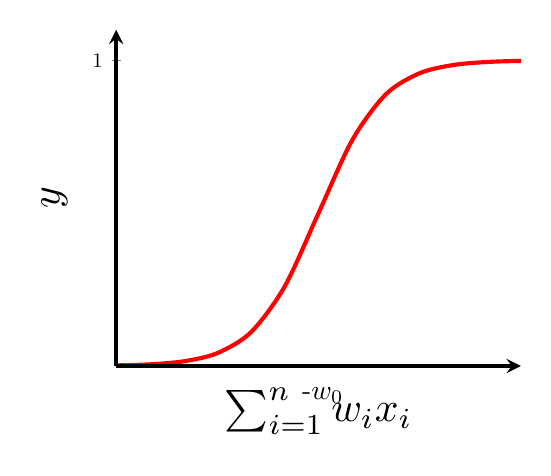
\begin{tikzpicture}[scale=0.75]
	\begin{axis}[
			xmin=-2.5, xmax=2.5,
			ymin=-0.0, ymax=1.1,
			axis lines=left,
			xtick=\empty, ytick={1},
			axis on top=true,
			line width = 2pt,
			%domain=-2.5:2.5,
			ylabel=$y$,
			xlabel=$\sum_{i=1}^{n} w_i x_i$,
			label style={scale=2}
		]
		\addplot [smooth,line width = 2pt, mark=none,draw=red] {1/(1+exp(-2.5*\x)};

		%% Add the asymptotes
	\end{axis}

	\node at (3.5,-0.5) {-$w_0$};
\end{tikzpicture}
				\vspace{0.1in}\\
				\onslide<2->{Smooth, continuous, \textbf{differentiable}}

			\end{center}
		\end{overlayarea}
	\end{columns}
\end{frame}
